\documentclass{svproc}
\usepackage{graphicx}
\usepackage{amsmath}
\usepackage{biblatex}
\usepackage{array}
\usepackage{longtable}
\usepackage{placeins}
\usepackage{float}
\usepackage{amssymb}
\usepackage{verbatim}
\usepackage{booktabs}
\usepackage[hidelinks]{hyperref}

\addbibresource{bib/lit.bib}

\title{LLaMA-Math: Quantized Optimization of Mathematical Reasoning}
\author{Simon Green\inst{1}}
\institute{
    School of Computing, University of Leeds, UK \\
    \inst{1} MSc, Artificial Intelligence \\
    \email{\{od21sg\}@leeds.ac.uk}
}
\date{\today}


%-----------------------------------------------------------------------

\begin{document}

\maketitle


%-----------------------------------------------------------------------


\begin{abstract}

This research introduces LLaMA-Math, a family of quantized, fine-tuned LLaMA 3.2 models optimized for mathematical reasoning, adapting DeepSeekMath’s Group-Relative Policy Optimization framework. Utilizing mathematical datasets—MATH, DeepMind Mathematics, NuminaMath, and Humanity’s Last Exam (HLE) for evaluation—we employ Quantized Low-Rank Adaptation to enable fine-tuning on a single GPU. We generate four fine-tuned versions, expecting improved accuracy and calibration on HLE’s rigorous reasoning tasks, particularly in novel problem-solving. By releasing source code, methodology, and the four fine-tuned open-source models, this work seeks to democratize large language model  fine-tuning and advance mathematical reasoning capabilities.

\keywords{GRPO, LLaMA, QLoRA, Fine-Tuning, Reinforcement Learning, HLE, Evaluation Metrics, Policy Optimization}

\end{abstract}


%-----------------------------------------------------------------------


\section{Introduction}

The rise of large language models (LLM) has transformed natural language processing, enabling unprecedented capabilities across diverse tasks. These systems, trained on vast corpora of text and multimedia assets, excel in recognizing and reproducing patterns within their training data. However, fine-tuning such models—adapting their billions of parameters to specialized domains—remains a significant challenge due to the computational cost and memory demands of traditional methods. These resource-intensive requirements often restrict fine-tuning to high-end infrastructure, limiting accessibility for researchers and practitioners with modest hardware. Recent innovations, however, suggest a shift in this landscape, promising that consumer-grade systems can customize state-of-the-art models effectively.

Among these advancements, Quantized Low-Rank Adaptation (QLoRA) has emerged as a transformative technique. By combining quantization, which reduces the precision of model weights, with low-rank adapters that update only a small subset of parameters, QLoRA significantly cuts memory requirements without compromising performance \cite{dettmers2023qloraefficientfinetuningquantized}. This approach has made it possible to fine-tune models with tens of billions of parameters on hardware as accessible as a single GPU, a capability previously unimaginable \cite{dettmers2023qloraefficientfinetuningquantized}. Concurrently, reinforcement learning strategies, such as the Group-Relative Policy Optimization (GRPO) algorithm introduced in the DeepSeekMath paper, have refined model optimization by focusing on relative rewards within groups, enhancing training efficiency and effectiveness \cite{shao2024deepseekmathpushinglimitsmathematical}.

Despite these strengths, LLMs often struggle with truly creative reasoning, a limitation evident when they are tasked with novel challenges beyond pattern recognition \cite{deutsch2011beginning}. This gap is starkly illustrated by Humanity’s Last Exam (Fig.~\ref{fig:hle_categories}) a dataset designed to probe creativity through 2,700 multimodal questions spanning mathematics, physics, philosophy, and natural sciences. Even top-performing models achieved a mere 14\% success rate on HLE, underscoring the need for advancements in reasoning capabilities \cite{phan2025humanitysexam}. In this study, we propose to address this challenge by integrating QLoRA and GRPO with a curated collection of mathematical datasets to fine-tune the open-weight LLaMA 3.2 model family. To our knowledge, this is the first study to evaluate LLaMA 3.2 on HLE and fine-tune it using QLoRA and GRPO, tackling both accessibility and reasoning limitations in LLMs.

\begin{figure}[H]
  \centering
  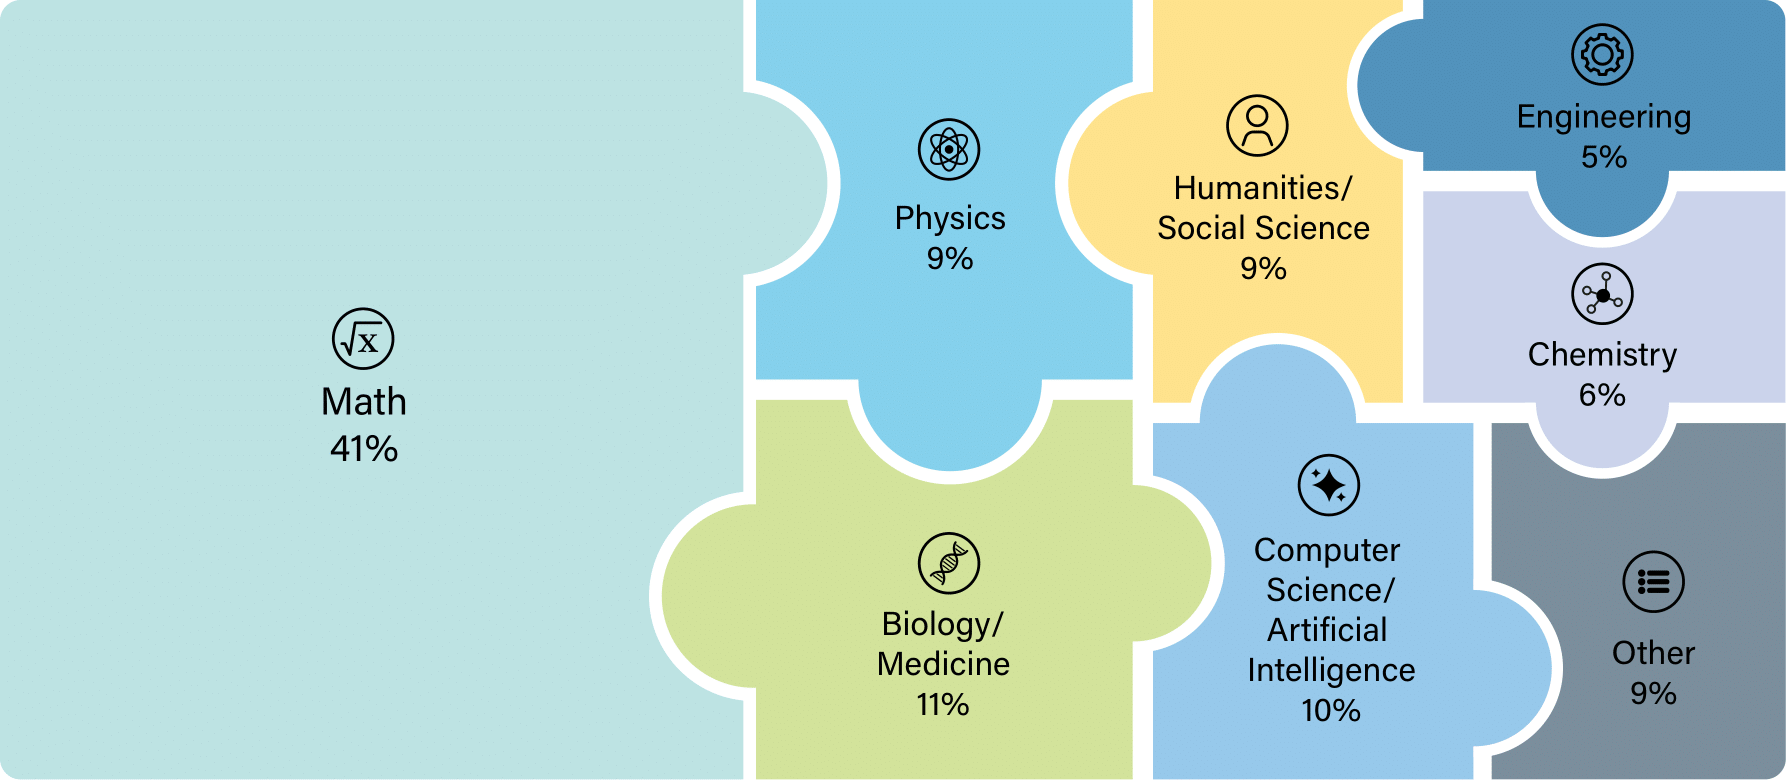
\includegraphics[width=0.8\textwidth]{.assets/dataset.png}
  \caption{HLE Dataset Categories \cite{phan2025humanitysexam}.}
  \label{fig:hle_categories}
\end{figure}

%-----------------------------------------------------------------------

\section{Literature Review and Research Hypothesis}

This study addresses the intertwined challenges of fine-tuning large language models, aiming to enhance accessibility for specialized applications and advance reinforcement learning’s role in improving reasoning capabilities. The open-weight nature of modern LLMs, coupled with their widespread adoption across domains like business, technology, and personal applications, positions them as a potentially transformative technology, comparable to the internet in societal impact. Yet, despite their ubiquity, personalizing or developing new models remains out of reach for most due to resource constraints and technical complexity \cite{dettmers2023qloraefficientfinetuningquantized}. This disparity highlights the urgent need for efficient, reliable methods that enable a broader range of stakeholders to adapt openly accessible technologies to their needs, democratizing innovation in this field.

Our research hypothesis emerges from two key questions. First, can a reinforcement learning approach—specifically GRPO combined with QLoRA and open-weight models—drive meaningful advancements in LLM reasoning capabilities? Second, does this methodology provide a practical pathway for diverse actors, including those with limited computational resources, to develop tailored models? These questions blend technical inquiry into model performance with a practical focus on broadening access, aligning with trends in efficient fine-tuning and scalable AI deployment \cite{dettmers2023qloraefficientfinetuningquantized}. We hypothesize that applying GRPO and QLoRA to LLaMA 3.2 will improve accuracy and calibration on mathematical reasoning tasks, enabling fine-tuning on a single GPU.

Our primary objective is to demonstrate the potential of combining model quantization with advanced RL techniques to elevate mathematical reasoning capabilities, without setting a specific numerical improvement threshold. This emphasis on methodological innovation prioritizes feasibility and scalability over arbitrary performance targets. A secondary objective is to evaluate the fine-tuned models’ performance on the HLE dataset, a benchmark of novel and challenging problems unseen during training \cite{phan2025humanitysexam}. We will assess generalization by evaluating accuracy, calibration, and error rates on HLE, focusing on novel problem-solving categories. This evaluation will shed light on the transferability of our fine-tuning strategy to uncharted domains, a key indicator of its robustness. Additionally, we propose that this RL-based methodology offers a reproducible framework for superior fine-tuning outcomes, serving as a practical alternative to resource-heavy training paradigms \cite{dettmers2023qloraefficientfinetuningquantized, shao2024deepseekmathpushinglimitsmathematical}.


%-----------------------------------------------------------------------


\section{Contributions and Knowledge Advancements}

We anticipate that this study will reinforce recent advances in reinforcement learning for fine-tuning language models. By leveraging GRPO to improve generalization to novel mathematical problems, as exemplified by the HLE dataset \cite{phan2025humanitysexam}, we aim to validate its effectiveness. Structuring our evaluation framework in line with the original HLE study ensures continuity with prior scholarship while pushing the boundaries of mathematical reasoning in LLMs. This work addresses a pressing scholarly need for adaptive models capable of tackling complex, unseen challenges, offering fresh insights into the synergy between RL techniques and mathematical problem-solving \cite{sutton2018reinforcement}.

As an intermediary step, we propose a pilot study to systematically explore the practical challenges of building a fine-tuning pipeline for large-scale models on a single GPU. These challenges encompass memory constraints, optimization inefficiencies, and the intricate tuning of hyperparameters when combining GRPO with QLoRA. Insights from this effort to operate on limited hardware will be thoroughly documented in our final report, providing the research community with a valuable resource for similar endeavors. This pilot phase will directly guide a subsequent phase, expanding to include the full suite of models and datasets targeted here. By openly sharing all project components, including source code, we empower researchers to use this baseline to test our methodology across diverse domains and scales.

A key contribution lies in the development and open dissemination of four fine-tuned models, optimized for mathematical reasoning, alongside evaluations of their four vanilla LLaMA 3.2 counterparts. These fine-tuned models, crafted through our pipeline, will be made publicly available on Hugging Face with comprehensive documentation and implementation guidelines. This release supports our goal of democratizing access to advanced reasoning models.

Additionally, this study underscores QLoRA’s efficacy as a strategy for training large-parameter models on a single device. By applying QLoRA to four LLaMA 3.2 variants, we will establish a performance benchmark against the HLE dataset. Demonstrating QLoRA’s ability to maintain computational efficiency without sacrificing performance will broaden access to advanced model training, particularly for researchers and institutions with limited infrastructure \cite{dettmers2023qloraefficientfinetuningquantized}.

Finally, this research enriches existing knowledge by offering a transparent, replicable application of the GRPO algorithm to LLM fine-tuning, inspired by the DeepSeekMath team’s pioneering work \cite{shao2024deepseekmathpushinglimitsmathematical}. Through this adaptation, we confirm GRPO’s effectiveness in enhancing mathematical reasoning and extend its applicability to diverse model architectures and evaluation frameworks. Our approach bridges theoretical progress with practical execution. Together, these contributions—methodological innovation, model release, and algorithmic application—lay a foundation for future RL-based fine-tuning advancements, enabling efficient, high-performing models for academic and practical use.

%-----------------------------------------------------------------------

\section{Pilot Study}

We fine-tune the LLaMA 3.2 1B Instruct model on a subset of the HLE dataset, selected for its low computational demands and focus on creative reasoning over retrieval, to validate our pipeline, quantify resource needs, and pinpoint barriers ahead.

\subsection{Dataset Analysis}

The HLE dataset, comprising 2,700 questions across eight categories, is detailed in Table~\ref{tab:dataset_description}\footnote{Available at \href{https://github.com/pre63/quantized-optimization-of-mathematical-reasoning-study/blob/main/pilot/analysis.ipynb}{Pilot Analysis Notebook}.}. Questions in \textit{Engineering}, \textit{Computer Science, AI}, and \textit{Math} unfold as expansive, intricate texts, with Math’s LaTeX-driven structure—e.g., \(\alpha + \beta = \gamma\)—producing a higher \(\mu\) due to its unique tokenization, unlike the denser, more uniform narratives of \textit{Social Sciences} and \textit{Humanities}, which show a lower \(\mu\) and narrower spread. For this pilot, we split the dataset approximately 60\% for training and 40\% for testing to ensure sufficient samples for robust evaluation across all categories, using a stratified split outlined in Table~\ref{tab:split_analysis} (minimum test sizes) and Table~\ref{tab:split_statistics} (counts and statistics). We assess the statistical significance of the minimum test size with:

\begin{equation}
  n = \frac{Z^2 \cdot p \cdot (1 - p)}{E^2},
\end{equation}

\noindent
where \(Z = 1.645\) (90\% confidence), \(p = 0.5\) (maximum variance), and \(E = 0.05\) (5\% error), adjusted for finite populations by:
\begin{equation}
  n_{\text{adjusted}} = \frac{n}{1 + \frac{n - 1}{\text{total examples}}},
\end{equation}

\noindent
yielding a test percentage of \(\left(\frac{n_{\text{adjusted}}}{\text{total examples}}\right) \times 100\).

\begin{center}
  \begin{table}[H]
\centering
\begin{tabular}{llll}
\toprule
Category & Text Tokens  & Image Size (MB) & Images \\
\midrule
Biology/Medicine & $\downarrow$11 - $\uparrow$3008 257.13$\mu$ $\pm$344.08$\sigma$ & 0.3582$\mu$ $\pm$0.3318$\sigma$ & 19.47\% \\
Chemistry & $\downarrow$16 - $\uparrow$1699 186.07$\mu$ $\pm$259.06$\sigma$ & 0.0655$\mu$ $\pm$0.0967$\sigma$ & 36.47\% \\
Computer Science/AI & $\downarrow$15 - $\uparrow$5052 420.34$\mu$ $\pm$648.82$\sigma$ & 0.2335$\mu$ $\pm$0.3776$\sigma$ & 5.81\% \\
Engineering & $\downarrow$14 - $\uparrow$8972 396.45$\mu$ $\pm$919.56$\sigma$ & 0.1733$\mu$ $\pm$0.2037$\sigma$ & 40.0\% \\
Humanities/Social Science & $\downarrow$15 - $\uparrow$1294 201.03$\mu$ $\pm$227.64$\sigma$ & 0.3205$\mu$ $\pm$0.3624$\sigma$ & 10.64\% \\
Math & $\downarrow$15 - $\uparrow$13518 216.81$\mu$ $\pm$483.85$\sigma$ & 0.145$\mu$ $\pm$0.211$\sigma$ & 4.07\% \\
Other & $\downarrow$11 - $\uparrow$7156 174.16$\mu$ $\pm$478.07$\sigma$ & 0.3883$\mu$ $\pm$0.4474$\sigma$ & 22.48\% \\
Physics & $\downarrow$11 - $\uparrow$7313 248.2$\mu$ $\pm$520.54$\sigma$ & 0.1423$\mu$ $\pm$0.253$\sigma$ & 5.83\% \\
\bottomrule
\end{tabular}
\vspace{0.2cm}
\caption{Dataset Description by Category for cais/hle Test Split}
\label{tab:dataset_description}
\end{table}

  \begin{table}[H]
\centering
\begin{tabular}{lrrrr}
\toprule
Category & Questions & Min Test Size & Min Test \% & Train \% \\
\midrule
Biology/Medicine & 303 & 143 & 47.260000 & 52.740000 \\
Chemistry & 170 & 105 & 61.560000 & 38.440000 \\
Computer Science/AI & 258 & 132 & 51.290000 & 48.710000 \\
Engineering & 130 & 88 & 67.720000 & 32.280000 \\
Humanities/Social Science & 235 & 126 & 53.630000 & 46.370000 \\
Math & 1106 & 218 & 19.670000 & 80.330000 \\
Other & 258 & 132 & 51.290000 & 48.710000 \\
Physics & 240 & 127 & 53.100000 & 46.900000 \\
\bottomrule
\end{tabular}
\vspace{0.2cm}
\caption{Statistics by Category for cais/hle Test Split (90\% CI, 5\% Error)}
\label{tab:split_analysis}
\end{table}

  \begin{table}[H]
\centering
\begin{tabular}{lrrrrr}
\toprule
Category & Questions & Train \% & Test \% & \% Image & \% Exact Match \\
\midrule
Biology/Medicine & 303 & 52.81 & 47.19 & 19.58 & 48.25 \\
Chemistry & 170 & 38.24 & 61.76 & 38.10 & 75.24 \\
Computer Science/AI & 258 & 48.84 & 51.16 & 6.82 & 69.70 \\
Engineering & 130 & 32.31 & 67.69 & 46.59 & 72.73 \\
Humanities/Social Science & 235 & 46.38 & 53.62 & 11.11 & 59.52 \\
Math & 1106 & 80.29 & 19.71 & 4.13 & 91.28 \\
Other & 258 & 48.84 & 51.16 & 22.73 & 75.00 \\
Physics & 240 & 47.08 & 52.92 & 6.30 & 84.25 \\
\bottomrule
\end{tabular}
\vspace{0.2cm}
\caption{Dataset Train/Test Split by Category}
\label{tab:split_statistics}
\end{table}

\end{center}


\subsection{Estimated Memory Requirements for Training}

Estimating memory requirements for fine-tuning the four LLaMA 3.2 variants entails analyzing GPU memory demands within our pipeline, which employs 4-bit quantization via Quantized Low-Rank Adaptation and Group-Relative Policy Optimization. The pilot study on the LLaMA 3.2 1B Instruct model established a baseline, requiring approximately 2.8 GB of GPU memory for a modest sequence length. This usage is modeled as:

\begin{equation}
  M_{\text{total}} = M_{\text{base}} + M_{\text{LoRA}} + M_{\text{opt}} + M_{\text{grad}} + M_{\text{act}},
\end{equation}

\noindent
where \(M_{\text{total}}\) represents total GPU memory, \(M_{\text{base}}\) is the quantized base model’s memory, \(M_{\text{LoRA}}\) covers LoRA adapters, \(M_{\text{opt}}\) accounts for optimizer states, \(M_{\text{grad}}\) includes gradients, and \(M_{\text{act}}\) reflects activations. This breakdown provides a foundation for scaling estimates across the 1B, 3B, 11B, and 90B variants, each with distinct parameter counts and sequence lengths.

To accommodate these models’ varying demands, we extend the equation to:

\begin{equation}
  M_{\text{total}} = (P \cdot Q_{\text{bits}} / 8) + (R \cdot L \cdot P_{\text{LoRA}}) + (O \cdot P_{\text{opt}}) + (G \cdot P_{\text{grad}}) + (A \cdot S \cdot B),
\end{equation}

\noindent
where \(P\) is the parameter count, \(Q_{\text{bits}}\) is quantization precision (4-bit), \(R\) and \(L\) are LoRA rank and adapted layers, \(P_{\text{LoRA}}\) is the LoRA parameter fraction, \(O\) and \(P_{\text{opt}}\) relate to optimizer memory, \(G\) and \(P_{\text{grad}}\) to gradients, \(A\) to activation memory per token, \(S\) to sequence length, and \(B\) to batch size. This formulation captures the interplay of model size, sequence length, and batch size, though system memory—driven by data handling and framework overhead—is observed separately and scales with complexity.

Table~\ref{tab:memory_requirements} details memory estimates for each variant, tailored to their designated sequence lengths—8,000 tokens for 1B and 3B, and 128,000 tokens for 11B and 90B—reflecting the HLE dataset’s demands. These figures incorporate typical QLoRA settings with 4-bit quantization and a modest LoRA rank, balancing GPU and system memory for single-GPU feasibility.

\vspace{-\baselineskip}
\begin{table}[H]
  \centering
  \begin{tabular}{lccccc}
    \toprule
    \textbf{Model} & \textbf{Params} & \textbf{GPU*} & \textbf{System*} & \textbf{Batch} & \textbf{Seq. Len.**} \\
    \midrule
    LLaMA 3.2 1B & 1B & 3.5 & 40 & 2 & 8 \\
    LLaMA 3.2 3B & 3B & 5.8 & 48 & 1 & 8 \\
    LLaMA 3.2 11B & 11B & 12.0 & 80 & 1 & 128 \\
    LLaMA 3.2 90B & 90B & 24.0 & 120 & 1 & 128 \\
    \bottomrule
  \end{tabular}
  \vspace{0.5em}
  \caption{Estimated Memory Requirements for Fine-Tuning LLaMA 3.2 Variants with QLoRA and GRPO.\\
  *Memory Values in GB. **Sequence Length in thousands of tokens.}
  \label{tab:memory_requirements}
\end{table}
\vspace{-\baselineskip}

The table reveals memory scaling trends: GPU usage rises with parameter count and sequence length, while system memory reflects increased data overhead. Smaller variants (1B, 3B) remain viable on modest GPUs with batch adjustments, whereas the 11B and 90B models, with their expansive 128k sequence lengths, push single-GPU limits—e.g., 24 GB for 90B aligns with high-end consumer hardware like an RTX 3090. These estimates balance accessibility with practical constraints, guiding resource planning and potential optimizations for larger models.

\subsection{Prototype Development and Initial Findings}

We have developed a prototype, available in the GitHub repository tied to this proposal, and tested its functionality. Initial evaluations of the vanilla LLaMA 3.2 1B Instruct model have begun, uncovering challenges that will shape our methodology. Discrepancies between theoretical expectations and practical outcomes—particularly in memory usage and training feasibility—have led us to devise an expanded audit of the HLE evaluation process, extending beyond the original study’s scope.

\subsection{Key Challenges}

Initial tests of the LLaMA 3.2 1B Instruct model on the HLE dataset reveal significant obstacles to accessible fine-tuning, spanning resource demands and model performance. These hurdles, detailed below, expose a gap between theoretical claims and practical realities:

\begin{itemize}
  \item \textbf{High Memory Demands}: Training requires 32 GB of system memory—far exceeding the 1.5 GB needed for inference and most consumer hardware limits—despite QLoRA’s efficiency claims \cite{dettmers2023qloraefficientfinetuningquantized}.
  \item \textbf{Prohibitive Training Costs}: A 5-day, \$750 USD run on an A100 (40 GB VRAM) via Google Colab\footnote{Fine-tuning configuration at \href{https://github.com/pre63/quantized-optimization-of-mathematical-reasoning-study/blob/main/pilot/grpo/config.py}{grpo/config.py}.} underscores the inaccessibility of competitive performance for resource-limited researchers.
  \item \textbf{Evaluation Errors}: Early evaluations showed false positives and negatives, with about 50\% of results erroneous, prompting a script to audit this issue’s depth\footnote{Audit script at \href{https://github.com/pre63/quantized-optimization-of-mathematical-reasoning-study/blob/main/pilot/grpo/audit.py}{grpo/audit.py}.}. Preliminary analysis suggests errors may stem from model limitations or evaluation framework flaws, not solely HLE’s difficulty. The full study will investigate these causes and refine the framework.
  \item \textbf{Long-Problem Limitations}: HLE’s lengthy problems challenge LLaMA, especially with derivations and sequences featuring similar characters. For example, in \(\frac{d}{dx} (x^n) = nx^{n-1}\), repeated variables confuse the model, while long binary strings—e.g., "010101000001000"—trigger repetitive predictions of initial characters. This aligns with known autoregressive model struggles with sustained, token-sparse complexity \cite{vaswani2023attentionneed}. The full study will explore mitigations like enhanced attention mechanisms.
\end{itemize}

\subsection{Conclusion}

This pilot equips the broader study with a validated pipeline and critical insights into dataset and resource realities. It steers us toward optimizing memory use, reducing training costs, and tailoring the approach to HLE’s unique demands, ensuring the full investigation achieves practical, scalable outcomes.

%-----------------------------------------------------------------------

\section{Methodology}

We fine-tune four LLaMA 3.2 variants for mathematical reasoning using MATH \cite{hendrycksmath2021} (12,500 problems), DeepMind Mathematics \cite{saxton2019analysingmathematicalreasoningabilities} (~36M pairs), and NuminaMath \cite{numina_math_datasets} (~1M pairs) for training, reserving the HLE dataset \cite{phan2025humanitysexam} (2,700 questions) for evaluation. Dataset analysis identifies challenging problems using classification methods (e.g., k-means, random forest) based on features like problem length, token density, and LaTeX complexity, limiting the training dataset to 24,700 samples across the variants. This limit balances resource constraints and problem diversity, determined by analyzing complexity and overlap across datasets. Samples are integrated and tokenized, prioritizing quality and variety. Fine-tuning employs GRPO \cite{shao2024deepseekmathpushinglimitsmathematical} and QLoRA with RL on A100 GPUs via Google Colab, generating four models:  four fine-tuned versions (GRPO+QLoRA). While A100s are used initially, pilot insights will inform optimizations for consumer-grade hardware, aligning with democratization goals. Evaluation on HLE uses NLTK for error parsing and SciPy for statistical significance against \cite{phan2025humanitysexam}, yielding accuracy and calibration metrics. Model weights and documentation are uploaded to Hugging Face for accessibility.

\begin{table}[H]
  \centering
  \begin{tabular}{lcccc}
    \toprule
    \textbf{Dataset} & \textbf{Size} & \textbf{Format} & \textbf{Source} & \textbf{Focus} \\
    \midrule
    MATH & 12,500 problems & LaTeX/LaTeX & \cite{hendrycksmath2021} & High-school math \\
    DeepMind Math & ~36M pairs & Text/Text & \cite{saxton2019analysingmathematicalreasoningabilities} & School-level exercises \\
    NuminaMath & ~1M pairs & LaTeX/LaTeX & \cite{numina_math_datasets} & Competition problems \\
    HLE (evaluation) & 2,700 questions & Text/LaTeX & \cite{phan2025humanitysexam} & Creative reasoning \\
    \bottomrule
  \end{tabular}
  \caption{Datasets for Fine-Tuning and Evaluation.}
  \label{tab:datasets}
\end{table}

\subsection{Model Details}

The LLaMA 3.2 family includes autoregressive models designed for efficiency and performance \cite{vaswani2023attentionneed}. Fine-tuning leverages their probabilistic token prediction, enhancing reasoning through GRPO’s relative reward optimization and QLoRA’s quantization, adapting them for mathematical tasks.

%-----------------------------------------------------------------------

\section{Results}

Table~\ref{tab:results} presents a comparative evaluation of models on the Humanity's Last Exam (HLE) benchmark, combining results from Phan et al. (2025) with our anticipated performance for the LLaMA 3.2 family. We plan to evaluate each in its baseline form and with our fine-tuning pipeline, anticipating incremental gains in accuracy and calibration as model size increases. These projections aim to position LLaMA 3.2 competitively against leading models on HLE’s rigorous reasoning tasks, with full results pending further study.

\begin{center}
  \begin{table}[H]
  \centering
  \begin{tabular}{lccc}
    \toprule
    Model                   & Accuracy (\%) ↑ & Calibration Error (\%) ↓ & Source \\
    \midrule
    GPT-4o                   & 3.1             & 92.3                      & \cite{phan2025humanitysexam} \\
    Grok-2                   & 3.9             & 90.8                      & \cite{phan2025humanitysexam} \\
    Sonnet 3.5               & 4.8             & 88.5                      & \cite{phan2025humanitysexam} \\
    Gemini Flash Thinking    & 7.2             & 90.6                      & \cite{phan2025humanitysexam} \\
    o1                       & 8.8             & 92.8                      & \cite{phan2025humanitysexam} \\
    DeepSeek-R1*             & 8.6             & 81.4                      & \cite{phan2025humanitysexam} \\
    o3-mini (medium)*        & 11.1            & 91.5                      & \cite{phan2025humanitysexam} \\
    o3-mini (high)*          & 14.0            & 92.8                      & \cite{phan2025humanitysexam} \\
    LLaMA-Math 1B*           & -               & -                         & This study \\
    LLaMA-Math 1B* + GRPO    & -               & -                         & This study \\
    LLaMA-Math 3B*           & -               & -                         & This study \\
    LLaMA-Math 3B* + GRPO    & -               & -                         & This study \\
    LLaMA-Math 11B           & -               & -                         & This study \\
    LLaMA-Math 11B + GRPO    & -               & -                         & This study \\
    LLaMA-Math 90B           & -               & -                         & This study \\
    LLaMA-Math 90B + GRPO    & -               & -                         & This study \\
    \bottomrule
  \end{tabular}
  \vspace{0.2cm}
  \caption{Comparative Evaluation of Models on the Humanity's Last Exam Benchmark.\\
   *Model is not multi-modal, evaluated on text-only subset. \\
   LLaMA 3.2 results are anticipated projections from this study, with full data pending evaluation.}
  \label{tab:results}
\end{table}
\end{center}

%-----------------------------------------------------------------------


\section{Conclusion and Future Work}
DeepSeekMath and their efficient Group-Relative Policy Optimization algorithm, combined with Quantized Low-Rank Adaptation, offer a promising pathway to democratize large language model fine-tuning. We believe that this methodology may offer other these benefits to other scientific domains.


%-----------------------------------------------------------------------


\section*{Acknowledgements}

The author acknowledges the support provided by the School of Computing at the University of Leeds and extends appreciation to the developers of QLoRA, GRPO, and the HLE dataset for their invaluable, publicly accessible resources. Grok 3 was utilized to assist in drafting this work, with careful adherence to ethical copyright principles and respect for the original authors’ contributions.


%-----------------------------------------------------------------------


\section*{Data Access Statement}

The code and results used in this study are openly accessible at {\it \href{https://github.com/pre63/quantized-optimization-of-mathematical-reasoning-study}{this repository}}. It contains all the scripts, configurations, and datasets analysis necessary to reproduce the experiments and validate the findings presented in this work.


%-----------------------------------------------------------------------


\printbibliography


%-----------------------------------------------------------------------


\end{document}
